\documentclass[12pt, twoside]{article}
\setcounter{secnumdepth}{4}
\usepackage[utf8]{inputenc}
\usepackage[english,russian]{babel}
\newcommand{\hdir}{.}
\usepackage{graphicx}
\usepackage{caption}
\usepackage{amssymb}
\usepackage{amsmath}
\usepackage{mathrsfs}
\usepackage{euscript}
\usepackage{upgreek}
\usepackage{array}
%\usepackage{theorem}
\usepackage{graphicx}
\usepackage{subfig}
\usepackage{caption}
\usepackage{color}
\usepackage{url}
\usepackage{cite}
\usepackage{geometry}
\usepackage{tikz,fullpage}
\usepackage{enumerate}
\usepackage{autonum}
\usepackage{enumitem}%
%\usepackage[unicode, pdftex]{hyperref}
\usepackage{comment}
\usepackage{titlesec}

\titleformat{\paragraph}[runin]{\normalfont\normalsize\bfseries}{}{0pt}{}
% объявляем новую команду для переноса строки внутри ячейки таблицы
\newcommand{\specialcell}[2][c]{%
  \begin{tabular}[#1]{@{}c@{}}#2\end{tabular}}
\newcommand{\bmatr}{{\mathbf{B}}}
\newcommand{\cmatr}{{\mathbf{C}}}
\newcommand{\hmatr}{{\mathbf{H}}}
\newcommand{\fmatr}{{\mathbf{F}}}
\newcommand{\mmatr}{{\mathbf{M}}}
\newcommand{\xmatr}{{\mathbf{X}}}
\newcommand{\pmatr}{{\mathbf{P}}}
\newcommand{\xmatrt}{{\tilde{\mathbf{X}}}}
\newcommand{\imatr}{{\mathbf{I}}}
\newcommand{\vmatr}{{\mathbf{V}}}
\newcommand{\wmatr}{{\mathbf{W}}}
\newcommand{\umatr}{{\mathbf{U}}}
\newcommand{\zmatr}{{\mathbf{Z}}}
\newcommand{\zmatrt}{{\tilde{\mathbf{Z}}}}
\newcommand{\Tmatr}{\mathbf{T}}
\newcommand{\lambdamatr}{{\mathbf{\Lambda}}}
\newcommand{\phimatr}{\mathbf{\Phi}}
\newcommand{\sigmamatr}{\mathbf{\Sigma}}
\newcommand{\thetamatr}{\boldsymbol{\Theta}}
\newcommand{\Ri}{\mathcal{R}}
\newcommand{\rk}{\mathfrak{r}}
\newcommand{\ab}{{\wm}}
\newcommand{\bb}{{\mathbf{b}}}
\newcommand{\cb}{{\mathbf{c}}}
\newcommand{\db}{{\mathbf{d}}}
\newcommand{\eb}{{\mathbf{e}}}
\newcommand{\fb}{{\mathbf{f}}}
\newcommand{\gb}{{\mathbf{g}}}
\newcommand{\hb}{{\mathbf{h}}}
\newcommand{\mb}{{\mathbf{m}}}
\newcommand{\pb}{{\mathbf{p}}}
\newcommand{\qb}{{\mathbf{q}}}
\newcommand{\rb}{{\mathbf{r}}}
\newcommand{\tb}{{\mathbf{t}}}
\newcommand{\ub}{{\mathbf{u}}}
\newcommand{\vb}{{\mathbf{v}}}
\newcommand{\wb}{{\mathbf{W}}}
\newcommand{\xb}{{\mathbf{x}}}
\newcommand{\xt}{{\tilde{x}}}
\newcommand{\xbt}{\tilde{{\mathbf{x}}}}
\newcommand{\yb}{{\mathbf{y}}}
\newcommand{\zb}{{\mathbf{z}}}
\newcommand{\zt}{{\tilde{z}}}
\newcommand{\zbt}{{\tilde{\mathbf{z}}}}
\newcommand{\mub}{{\boldsymbol{\mu}}}
\newcommand{\alphab}{{\boldsymbol{\alpha}}}
\newcommand{\thetab}{{\boldsymbol{\theta}}}
\newcommand{\iotab}{\boldsymbol{\iota}}
\newcommand{\zetab}{\boldsymbol{\zeta}}
\newcommand{\xib}{\boldsymbol{\xi}}
\newcommand{\xibt}{\tilde{\boldsymbol{\xi}}}
\newcommand{\xit}{\tilde{\xi}}
\newcommand{\betab}{{\boldsymbol{\beta}}}
\newcommand{\phib}{{\boldsymbol{\phi}}}
\newcommand{\psib}{{\boldsymbol{\psi}}}
\newcommand{\gammab}{{\boldsymbol{\gamma}}}
\newcommand{\lambdab}{{\boldsymbol{\lambda}}}
\newcommand{\varepsilonb}{{\boldsymbol{\varepsilon}}}
\newcommand{\pib}{{\boldsymbol{\pi}}}
\newcommand{\sigmab}{{\boldsymbol{\sigma}}}
\newenvironment{comment}{}{}



\newcommand{\scl}{s_{\mathsf{c}}}
\newcommand{\shi}{s_{\mathsf{h}}}
\newcommand{\shib}{\mathbf{s}_{\mathsf{h}}}
\newcommand{\MOD}{M}
\newcommand{\entr}{\mathsf{H}}
\newcommand{\REG}{\Omega}
\newcommand{\Mquol}{V}
\newcommand{\prob}{p}
\newcommand{\expec}{\mathsf{E}}

\newcommand{\xo}{{\overline{x}}}
\newcommand{\Xo}{{\overline{x}}}
\newcommand{\yo}{{\overline{y}}}

\newcommand{\xbo}{{\overline{\mathbf{x}}}}
\newcommand{\Xbo}{{\overline{\mathbf{X}}}}

\newcommand{\Amc}{{\mathcal{A}}}
\newcommand{\Bmc}{{\mathcal{B}}}
\newcommand{\Cmc}{{\mathcal{C}}}
\newcommand{\Jmc}{{\mathcal{J}}}
\newcommand{\Imc}{{\mathcal{I}}}
\newcommand{\Kmc}{{\mathcal{K}}}
\newcommand{\Lmc}{{\mathcal{L}}}
\newcommand{\Mmc}{{\mathcal{M}}}
\newcommand{\Nmc}{{\mathcal{N}}}
\newcommand{\Pmc}{{\mathcal{P}}}
\newcommand{\Tmc}{{\mathcal{T}}}
\newcommand{\Vmc}{{\mathcal{V}}}
\newcommand{\Wmc}{{\mathcal{W}}}
\newcommand{\Smi}{{\mathcal{S}}}

\newcommand{\T}{^{\text{\tiny\sffamily\upshape\mdseries T}}}
\newcommand{\deist}{\mathbb{R}}
\newcommand{\ebb}{\mathbb{E}}

\newcommand{\Amatr}{\wm}
\newcommand{\X}{\mathbf{X}}
\newcommand{\Z}{\mathbf{Z}}
\newcommand{\Umatr}{\mathbf{U}}
\newcommand{\zetavec}{\boldsymbol{\zeta}}

\newcommand{\M}{\mathbf{M}}
\newcommand{\x}{{\mathbf{x}}}
\newcommand{\z}{{\mathbf{z}}}
\newcommand{\ical}{{\mathcal{I}}}
\newcommand{\tvec}{{\mathbf{t}}}
\newcommand{\xvec}{{\mathbf{x}}}
\newcommand{\zvec}{{\mathbf{z}}}
\newcommand{\bvec}{{\mathbf{b}}}
\newcommand{\qvec}{{\mathbf{z}}}
\newcommand{\pvec}{{\mathbf{p}}}
\newcommand{\wvec}{{\mathbf{W}}}
\newcommand{\rvec}{{\mathbf{r}}}
\newcommand{\thetavec}{{\mathbf{\theta}}}
\newcommand{\y}{{\mathbf{y}}}
\newcommand{\g}{{\mathbf{g}}}
\newcommand{\w}{{\mathbf{W}}}
\newcommand{\wm}{{\mathbf{w}}}
\newcommand{\m}{{\mathbf{m}}}


\newtheorem{theorem}{Теорема}
\newtheorem{definition}{Определение}
\DeclareMathOperator*{\argmin}{arg\,min}
\graphicspath{ {pics/} }
%\graphicspath{ {fig/} }
\begin{document}
\selectlanguage{russian}
\title{\textbf{Аддитивная регуляризация и ее метапараметры при выборе структуры сетей глубокого обучения}\thanks{Работа выполнена при поддержке РФФИ (проекты 19-07-1155, 19-07-0885) и правительства РФ (соглашение 05.Y09.21.0018). Настоящая статья содержит результаты проекта <<Статистические методы машинного обучения>>, выполняемого В~рамках реализации Программы Центра компетенций Национальной технологической инициативы <<Центр хранения и анализа больших данных>>, поддерживаемого Министерством науки и высшего образования Российской Федерации по Договору МГУ им.\,М.\,В.\,Ломоносова  с Фондом поддержки проектов Национальной технологической инициативы от 11.12.2018 № 13/1251/2018.}}
\date{}
\maketitle

\begin{center}
\bf
М.\,С.~Потанин\footnote{Московский физико-технический институт, mark.potanin@phystech.edu}, К.\,О.~Вайсер\footnote{Московский физико-технический институт, vajser.ko@phystech.edu},  В.\,В.\,Стрижов\footnote{Вычислительный центр имени А.\,А.\,Дородницына Федерального исследовательского центра <<Информатика и управление>> Российской академии наук; Московский физико-технический институт, strijov@phystech.edu}
\end{center}

\begin{abstract}	
Решается задача выбора модели глубокого обучения. Выбор оптимизации функции ошибки. Включение аддитивной регуляризации. Сеть глубокого обучения представима в виде суперпозиции автокодировщика и нейронной сети. Под сложностью модели понимается мера множества допустимых значений параметров.
Функция аддитивной регуляризации это линейная комбинация экпертно заданных регуляризаторов. Веса слагаемых есть метапараметры. Исследуются свойства алгоритма оптимизации метапараметров аддитивной регуляризации.  Исследуются зависимости точности, сложности и устойчивости модели от метапарметров аддитивной регуляризации.
\end{abstract}

{\bf Ключевые слова:} автокодировщик; нейронные сети; структура; аддитивная регуляризация.

\setcounter{secnumdepth}{0}
\section{Введение}


В данной работе рассматривается влияние способа построения функции ошибки на выбор структуры сети глубокого обучения. Функция ошибки~---это оценка качества модели. Сеть оптимальной структуры как можно более точно аппроксимирует исходную неизвестную зависимость целевой переменной $y$ от векторов признакового пространства $\xb$. Моделью называется отображение $f:(\xb,\wm)\mapsto y$. В общем виде модель глубокого обучения представляет собой суперпозицию обобщенных линейных моделей и выглядит как \eqref{eq:model}. Такая модель может содержать большое число слоев и нейронов. Под структурной сложностью модели понимается число параметров модели. Предполагается, что чем сложнее модель, тем выше у нее точность аппроксимациии, то есть тем меньше значение функции ошибки. Однако увеличение сложности модели приводит к снижению ее устойчивости, то есть зависимости результата от изменения начальных данных (сюда ссылку про это). Предлагается разработать метод, позволяющий понизить сложность модели при сохранении ее точности. В работе --(прошлая статья)-- поиск структуры работал через добавление или удаление элементов из структуры генетическим алгоритмом. Это решение по сути являлось разновидностью полного перебора. В этой работе также предлагается использовать аддитивную регуляризацию для выбора оптимальной структуры. 

\begin{comment}
    Требуется предложить стратегию направленного поиска. Такая стратегия, конечно, работает чуть хуже чем полный перебор. 
Алгоритм градиентного спуска сходится довольно быстро. Требуется исследовать возможность поиска оптимальной структуры через сложность. 
\end{comment}


Задачи, решение которых не существует, не единственно или не устойчиво, принято называть \textit{некорректно поставленными по Адамару}\cite{tikhonov1977solutions}.
\begin{definition}%{Regularization}
Регуляризация~---метод решения задач, в котором для выбора оптимального решения задаются дополнительные критерии
оптимальности, учитывающие специфические требования решаемой задачи и называемые регуляризаторами. 
\end{definition}
\begin{definition}%{ Additive Regularization}
Аддитивная регуляризация~---это вид регуляризации, основанный на оптимизации взвешенной суммы регуляризаторов. 
\end{definition}
Регуляризация повышает устойчивость прогноза в случае мультикореллированости параметров модели или переменных признакового пространства. Она способствует повышению обобщающей способности модели и снижению риска переобучения \cite{svensen2007pattern}. Регуляризация предотвращает ситуацию, когда параметры становятся константными и не изменяются в процессе оптимизации модели.

В качестве объекта исследования выступает способ построения функции ошибки. Аддитивная регуляризация имеет вид \eqref{eq:error_function}. Исследуется влияние весов регуляризаторов  \eqref{regularization_sum} на сложность и точность модели.
Аддитивная регуляризация записывается как
\begin{equation}\label{regularization_sum}
\sum\limits_{i=1}^r \mathbf{\lambda}_i^T\mathcal{R}_i,    
\end{equation}
где $\mathcal{R}_i$~---регуляризатор.
\begin{definition}%{Metaparameters}
Метапараметры~---веса регуляризаторов, используемые для оптимизации параметров модели.
\end{definition}
Веса регуляризаторов в данной работе изменяются в ходе процедуры оптимизации. Это изменение называется расписанием оптимизацию.
Для этого составляется расписание оптимизации метапараметров $\mathbf{\lambda}$ аддитивной регуляризации. В отличие от регуляризации для линейных моделей, метапарамеры аддитивной регуляризации назначаются для каждого из слоев нейронной сети. 

Например, элемент функции ошибки с аддитивной регуляризацией может иметь следующую структуру:
\[\lambda \|L\wm\|_2^2,\]
где $\lambda$ ~--- метапараметр функции ошибки, $L$ ~--- гиперпараметр модели, $\wm$ ~--- параметр модели.


\begin{definition}%{Hyperparameters}
Гиперпараметры~---параметры функции аддитивной регуляризации, используемые для оптимизации параметров модели и метапараметров. В этой работе гиперпараметры считаются экспертно заданными, неизменяемыми параметрами. Они являются элементами функции ошибки.
\end{definition}

Варьирование значений метапараметров добавляет и удаляет из рассмотрения различные регуляризаторы. В функцию ошибки добавляются индивидуальные регуляризаторы для каждого слоя нейросети.

Алгоритм оптимизации параметров модели состоит следующих шагов ~--- 
1) экспертное задание гиперпараметров модели, 2) оптимизация параметров модели
, 3) оптимизация метапараметров модели. Параметры модели оптимизируются алгоритмом обратного распространения ошибки. Оптимизация метапараметров происходит с помощью генетического алгоритма.



\section{Обзор литературы}

Регуляризация $L_2$ работает с помощью установления баланса между смещением и дисперсией. Но ее недостаток в том, что она не может создать разреженную модель, так как сохраняет все множество параметров. Другой вид регуляризации $L1$ был предложен в \cite{tibshirani1996regression}, и он предлагает автоматический выбор параметров. Но он также имеет несколько недостатков, среди которых:
\begin{enumerate}
\item[1)]
Если обозначить за $p$ число независимых переменных, а за $n$ количество объектов в выборке, то в случае $p>n$ lasso регуляризация выбирает максимально $n$ независимых переменных из множества.
\item[2)]
При наличии групп сильно скоррелированных переменных, lasso регуляризация выбирает только одну переменную из группы, причем не обращая внимания какую именно.
\item[3)]
В случае $n>p$ и наличии высокой корреляции между переменными было эмпирически показано, что ridge регрессия работает намного лучше lasso.
\end{enumerate}
Таким образом, пукнты 1) и 2) делают lasso неприменимой техникой в некоторых задачах, где требуется отбор признаков. Перечисленные проблемы решаются с помощью другой техники регуляризации elastic net \cite{zou2005regularization}, которая позволяет производить автоматический отбор переменных, регулировать их веса, а так же выбирать группы коррелярующих признаков. Метод регуляризации elastic net представляет собой добавление в функцию ошибки двух дополнительных слагаемых
\begin{equation}
S(\lambda_1,\lambda_2,\lambda_3,\wm) = \lambda_1|\yb-\xmatr\wm|^2+\lambda_2|\wm|^2+\lambda_3|\wm|_1
\end{equation}

Обобщением elastic net является регуляризация Support Features Machine. Функция ошибки  задается в виде
\begin{equation}\label{eq:SVM}
\underset{\mathbf{w},\mathbf{w_0}}\min\quad L (\wm, \mathbf{w_0}) C\sum_{i=1}^l(1 - M_i(\mathbf{w},\mathbf{w_0}))_+ + \sum_{i=1}^nR_{\mu}(w_j),
\end{equation}
\begin{equation}
R_{\mu}(w_j) = \begin{cases}
2\mu|w_j|,& |w_j| \leq \mu, \\
\mu^2 + w_j^2,& |w_j| \geq \mu. \\
\end{cases}
\end{equation}
Признаки отбираются с помощью параметра селективности $\mu$. Шумовые признаки ($|w_j| < \mu$) подавляются как и в Lasso, а значимые зависимые признаки группируются также как и в elastic net.
На нее похож такой метод как Relevance Features Machine. Задается в виде
\begin{equation}\label{eq:RFM}
\underset{\mathbf{w},\mathbf{w_0}}\min\quad C\sum_{i=1}^l(1 - M_i(\mathbf{w},\mathbf{w_0}))_+ + \sum_{i=1}^n\ln(w_j^2 + \frac{1}{\mu})
\end{equation}
Отличие \eqref{eq:RFM} от метода \eqref{eq:SVM} в том, что происходит более совершенный отбор признаков, когда они только совместно обеспечивают хорошее решение.

В общем случае, если функция $L$~--- выпуклая, то можно воспользоваться регуляризацией Moreau-Yosida. Записывается  $\lambda > 0$
\begin{equation}
M_{\lambda L}(x) = \underset{u}\inf(L(u) + \frac{1}{2\lambda}||x - u||_2^2) 
\end{equation}
У этой функции ряд замечательных свойств~---1) $M_{\lambda f}(x)$~--- выпуклая функция в силу инфимальной конволюции; 2) множество точек минимума для $L$ и $M_{\lambda L}(x)$ совпадают; 3) $M_{\lambda L}(x)$~--- гладкая функция в силу сильной выпуклости ее первой сопряженной функции и совпадении со второй сопряженной функцие $M_{\lambda L}(x) = M_{\lambda L}^{**}(x)$. \\

В статье \cite{haber2017stable} представлены несколько стратегий стабилизации оптимизации структуры очень глубоких сетей. Они основаны на системах обыкновенных дифференциальных уравнений (ODE). Так же в этой статье вводят регуляризацию, чувствительную к плавному изменению параметров модели между соседними слоями. Кроме того, как показано в численных экспериментах, регуляризация повышает устойчивость модели. 

\begin{comment}
    Важность такого вида регуляризации иллюстрирует следующий пример - рассматривается удаление одного слоя из глубокой сети. Поскольку сеть глубокая, не следует ожидать больших изменений значений выходного слоя и, следовательно, ошибок классификации. Однако, если этот слой выполняет, например, поворот элементов на 90 градусов, в то время как соседние слои сохраняют элементы без изменений, эффект будет существенным.
\end{comment}

Для практического использования аддитивной регуляризации важно, чтобы помимо высокой точности аппроксимации целевой функции модель являлась бы интерпретируемой. Например, исследования показали, что в области медицины предпочитаются модели основанные на деревьях решений, из-за того, что можно проследить,на основании каких правил строился прогноз. Тем не менее, возможность узнать причины предсказаний модели не являтся основным критерием применимости модели. Если эти причины  расходятся со здравым смыслом и экспертными правилами данной области, то такая модель не является приемлемой. Эти два критерия называются интерпретируемостью и точностью аппроксимации модели.

В работе \cite{wang2018learning} авторы рассматривают новый способ регуляризации EYE (expert yielded estimates), который включает в себя экспертные знания об отношениях между признаками и зависимой переменной. Авторы расматривают задачу минимизации эмпирического риска
\begin{equation}\label{eq1}
\hat{\mathbf{\w}} = \argmin\text{S}(\w,\X,\mathbf{y})+n\lambda\mathcal{J}(\w,\mathbf{\Gamma})
\end{equation}
в которой минимизируется сумма функции ошибки и регуляризации $\mathcal{J}$. Имеется множества признаков $\mathcal{D}$, из которых для множества $\mathcal{K}\subseteq\mathcal{D}$ имеется дополнительная информация о том, что эти признаки являются важными в рассматриваемой экспертной области. Следовательно для $\hat{\mathbf{\w}}_{\mathcal{D}\setminus\mathcal{K}}$ требуется разреженность, а для $\hat{\mathbf{\w}}_{\mathcal{K}}$~---нет. Базовый подход, используемый авторами, заключается в использовании $L1$ и $L2$ регуляризаций, тогда регуляризационный член имеет вид
\begin{equation}\label{eq2}
\mathcal{J} = (1-\beta)||\mathbf{\Gamma}\odot\w||^2_2+\beta||(1-\mathbf{\Gamma})\odot\w||_1,
\end{equation}
где параметр $\beta$ контролирует баланс между признаками из $\mathcal{K}$ и $\mathcal{D}\setminus\mathcal{K}$. Предлагаемое авторами решение имеет следующий вид
\begin{equation}\label{eq3}
\mathcal{J} = ||(1-\mathbf{\Gamma})\odot\w||_1 + \sqrt{ ||(1-\mathbf{\Gamma})\odot\w||^2_1+||\mathbf{\Gamma}\odot\w||^2_2}.
\end{equation}
Его  использование в задачах стратификации риска пациентов позволило получить модели, в которых основные используемые признаки сильно пересекались с факторами, которые считаются значимыми в медицинской среде. При э том удалось сохранить высокое качество предсказания.

\section{Постановка задачи}
\paragraph{Мотивация}
Для решения задачи выбора модели предлагается построить модифицированную функцию ошибки.
Требуется исследовать способ построить вид функции ошибки аддитивной регуляризации и ее влияние на точность и сложность модели глубокого обучения.

\paragraph{Выбор модели}
Задана выборка, конечное множество пар
\begin{equation}\label{eq3}
(\xb,y) \in D,\quad \xb \in \mathbb{R}^{n},\quad y\in \mathbb{R},
\end{equation}
где $\xb$~--- вектор независимых переменных, $y$~--- зависимая переменная. Моделью называется отображение $f:(\xb,\wm)\mapsto y$. Требуется построить аппроксимирующую модель $f(\x)$ вида:
\begin{equation}\label{eq:model}
f = \sigma_k\circ\underset{1\times1}{\wm_k^\mathsf{T}\sigmab_{k-1}}\circ\w_{k-1}\sigmab_{k-2}\circ\dots\circ\underset{n_2 \times 1}{\w_2\sigmab_1}\circ\underset{n_1 \times n}{\w_1}\underset{n \times 1}{\x}.
\end{equation}
Эта модель рассматривается как суперпозиция линейной модели, глубокой нейросети и автоэкнодера.
\\

\paragraph{Структура сети.}
В работе ==[прошлая статья]== рассматривается задача оптимизации структуры сети $\Gammab$ генетическим алгоритмом. Предлагается  использовать тот же подход и в текущей статье с добавлением аддитивной регуляризации. 

Решается задача выбора оптимальной структуры модели
\begin{equation}\label{eq57}
f = \sigma_k\circ\boldsymbol{\Gamma}_k\otimes\underset{1\times1}{\wm_k^\mathsf{T}\sigmab_{k-1}}\circ\boldsymbol{\Gamma}_{k-1}\otimes\w_{k-1}\sigmab_{k-2}\circ\dots\circ\boldsymbol{\Gamma}_2\otimes\underset{n_2 \times 1}{\w_2\sigmab_1}\circ\boldsymbol{\Gamma}_1\otimes\underset{n_1 \times n}{\w_1}\underset{n \times 1}{\x},
\end{equation}
где $\boldsymbol{\Gamma}$~---~ матрица, задающая структуру модели; $\otimes$~--- адамарово произведение, определяющееся как поэлементное умножение. Если элемент $\gamma\in\{0,1\}$ матрицы $\boldsymbol{\Gamma}$ равен нулю, то соответствующий элемент матрицы параметров $\w$ обнуляется, и не участвует в работе модели. Множество индексов соответствующих ненулевым элементам матрицы $\boldsymbol{\Gamma}$ обозначается $\mathcal{A}$.  Требуется найти такое подмножество индексов $\mathcal{A}^{*}$, которое доставляет минимум функции:
\begin{equation}\label{eq46}
\mathcal{A}^{*} = \arg \underset{\mathcal{A} \subseteq \mathcal{I}}\min L(f_{\mathcal{A}}|\wm^*, \mathfrak{D}_\mathcal{C}),
\end{equation}
на разбиении выборки $\mathfrak{D}$, определенным множеством индексов $\mathcal{C}$. Здесь $\mathcal{I} = \mathcal{C}\sqcup \mathcal{L}$~---~ все индексы всех матриц $\boldsymbol{\Gamma}$. То есть требуется снизить число признаков и повысить устойчивость модели.

При этом параметры $\textbf{w}^*$ модели доставляют минимум ошибки:
\begin{equation}\label{eq102}
\textbf{w}^* = \arg \underset{\textbf{w}}\min L(\textbf{w}|\mathfrak{D}_\mathcal{L}, f_\mathcal{A}),
\end{equation}
на разбиении выборки, определенной множеством $\mathcal{L}$.
Алгоритм поиска оптимальной структуры сети предполагает минимизацию функции ошибки.
\paragraph{Функция ошибки и критерии качества модели.}

Ключевой идеей данной работы является построение новой функции ошибки с использованием метапараметров аддитивной регуляризации. Предлагается использовать композитную функцию ошибки. Она состоит из нескольких слагаемых. Первое слагаемое соответствует точности восстановления зависимой переменной. Второе слагаемое это точность реконструкции независимой переменной автокодировщиком. Остальные $k$ слагаемых отвечают за аддитивную регуляризацию. Создается каталог слагаемых функции ошибки для построения аддитивной регуляризации.
\begin{table}[h!]
\begin{center}
\begin{tabular}{|c|c|}
\hline
   Роль в аддитивной регуляризации & Тип регуляризатора  \\
  \hline
  Ошибка выхода нейронной сети  & $||\mathbf{y} - f(\w)||^2_2 $   \\
  \hline
  Ошибка восстановления на каждом слое & $||\xb-\mathbf{r}(\xb)||^2_2$ \\
  \hline
  $L_1$ и $L_2$ регуляризация & $||\wm-\wm_0||_1$, $||\wm-\wm_0||^2_2$ \\
  \hline
  \begin{tabular}{c}
       Штраф за отличие матрицы одного слоя \\
       от тождественного преобразования
  \end{tabular}
   & $||\w-\mathbf{I}||$  \\
  \hline
  \begin{tabular}{c}
       Штраф за отличие матрицы одного слоя \\
       от метода главных компонент
  \end{tabular}
  & $||\w\w^T-\mathbf{I}||$ \\
  \hline
  Тихоновская регуляризация & 
  $\|\mathbf{T}\w\|$  \\
  \hline
\end{tabular}
\caption{Каталог регуляризаторов аддитивной функции ошибки}
\end{center}
\end{table}

Подробное рассмотроение типов используемых регуляризаторов представлено в Supplementary

Задача \eqref{eq:criterion_argmin} является задачей минимизации функции $L$, включающая слагаемое \eqref{eq:mce} и \eqref{eq:autoencoder_error} для оптимизации параметров модели \eqref{eq:model}
\begin{equation}\label{eq:error_function}
L = \lambda_xE_{\xb} + \lambda_yE_{\y} + \lambda_1\mathcal{R}_1+\dots+\lambda_k\mathcal{R}_k = \lambda_xE_x + \lambda_yE_y + \sum\limits_{i = 1}^k\mathbb{\lambda}_i \mathcal{R}_i(\mathbf{W}),
\end{equation}
где $\mathcal{R}_i = \mathcal{R}(\mathbf{W}) = (\rk_1(\mathbf{W}), \cdots , \rk_r(\mathbf{W}))^{\T}$~---вектор, состоящий из значений регуляризаторов $i$-ого слоя.%\begin{enumerate}
%\item[1)]
%$||\mathbf{y} - f(\w)||^2_2 = E_y$,
%\item[2)]
%$||\xb-\mathbf{r}(\xb)||^2_2$,
%\item[3)]
%$||\wm-\wm_0||_1$,
%$||\wm-\wm_0||^2_2$,
%\item[4)]
%$||\w-\mathbf{I}||$,
%\item[5)]
%$||\w\w^T-\mathbf{I}||$,
%\end{enumerate}
 Метапараметры аддитивной регуляризации представляют себя матрицу размером $k\times r$, где $k$~---число слоев, а $r$~---число регуляризаторов в каждом слое:
\[
\begin{bmatrix}
\lambda_{1,1}& \lambda_{1,2}&\dots&\lambda_{1,r}\\
\dots& \dots&\dots&\dots \\
\lambda_{k,1}& \lambda_{k,2}&\dots&\lambda_{k,r}
\end{bmatrix}.
\]
В свою очередь $\boldsymbol{\lambda}_i$ представляет собой вектор
\begin{equation}\label{eq4}
\mathbf{\lambda_k} = \left[\lambda_1,\lambda_2,\dots,\lambda_r \right].
\end{equation}
Каждый элемент этого вектора соответствует регуляризатору соответствующего слоя.
Подобный подход позволяет варьировать структуру функции ошибки. Например,если занулить ошибки $E_y$ и аддитивную регуляризацию, оставив только ошибку $E_x$ в функции \eqref{eq:error_function}, то слой будет вести как автокодировщик. Или наоборот, при слабой регуляризации параметра $E_y$ получится нейросетевой слой.

\begin{comment}
В работе \cite{bib_1} представлена таблица свойств различных регуляризаций. В работе рассматриваются нормы со степенью один и два, то есть метрики $L1$ и $L2$. Требуется исследовать свойства метрика с различными значениями степени. 
\end{comment}

При оптимизации структуры Г модели глубокого обучения используется три вида критериев качества: точность, устойчивость и сложность.

\paragraph{Точность.}

Когда в качестве используемой модели выступает нейросеть или линейная регрессия, 
то функция ошибки имеет вид:
\begin{equation}\label{eq:mce}
E_y= \sum_{((\xb,y) \in D)\in\mathcal{I}}\big(y-f(\xb)\big)^2.
\end{equation}
Эта функция ошибки включает в себя полученные предсказания модели и значения зависимых переменных. В задачах регрессии точность аппроксимации имеет вид: 
\begin{equation}\label{eq106}
\text{MAE} =\frac{ \sum\limits_{(\xb,y) \in D}|y-f(\xb)|}{|D|}.
\end{equation}

При включении в модель \eqref{eq:model} метода главных компонент или автокодировщика, метки объектов не используются. Функция ошибки штрафует невязки восстановленного объекта:
\begin{equation}\label{eq:autoencoder_error}
E_\mathbf{x} = \sum_{i\in\mathcal{I}}\left\Vert{\xb_i-\mathbf{r}(\xb_i)}\right\Vert_2^2,
\end{equation}
где $\mathbf{r}(\x)$  это линейная реконструкция объекта $\x$. 
Параметры автокодировщика
\begin{equation}
\textbf{W}_{\text{AE}} = \{\w^{'},\w,\mathbf{b}^{'},\mathbf{b}\}
\end{equation}
оптимизированы таким образом (\ref{eq:autoencoder_error}), чтобы приблизить реконструкцию $\mathbf{r}(\x)$ к исходному вектору $\x$.



\paragraph{Сложность.}\label{complexity}
Введем отношение порядка $\succ$ на множестве значений сложности. Это отношение задается множеством параметров модели:
\begin{enumerate}
\item[1)] один параметр: $w\in \mathbb{R}^1 \succ w \in \lambda_1 [0,1] +\lambda_0 \succ w\in c +\lambda_0$,
\item[2)] вектор(нейрон): $\wm\in \mathbb{R}^n \succ \left\Vert \wm \right\Vert^2 =1 \succ \wm= \text{const}$,
\item[3)] матрица(слой): $\wvec\in \mathbb{R}^{c{\times}n} \succ \wvec^\mathsf{T}\wvec = \mathbf{I} \succ \wvec= \text{const}$.
\end{enumerate}

Множество, которому принадлежит сложность модели – порядковое. Исходя из введенного понятия сложности модели упорядочены 
по возрастанию сложности:
\begin{enumerate}
\item[1)] линейная регрессия,  $\sigma^{'} = \text{id}, \sigma = \text{id}, \w = \mathbf{I}_n $ ,
\item[2)] линейная регрессия и метод главных компонент, $\sigma^{'} = \text{id}, \w^\mathsf{T}\w = \mathbf{I}_n $ ,
\item[3)] линейная модель и автокодировщик, $\w^\mathsf{T}\w \neq \textbf{I}_n$,
\item[4)] линейная модель и стэк автокодировщиков, представимый в виде суперпозиции~\eqref{eq:model},
\item[5)] двухслойная нейронная сеть,
\item[6)] глубокая нейронная сеть.
\end{enumerate}



\paragraph{Устойчивость~---}это минимум дисперсии функции ошибки \eqref{eq3}:
\begin{equation}\label{eq103}
\mathsf{D}(S) \rightarrow \min.
\end{equation}
\paragraph{Формулировка задачи}
Таким образом, задача сводится к следующему виду:
\begin{equation}\label{eq:criterion_function}
L(\wm,\mathbf{\lambda}) = E_{\yb} + E_{\xb} +
\sum\limits_{i = 1}^r\mathbb{\lambda}_i^T\mathcal{R}(\mathbf{W}_i)
\end{equation}
\begin{equation}\label{eq:criterion_argmin}
\begin{array}{r@{}l}
\wm= \arg \min L(f| \mathbf{\lambda}, \mathbf{\Gamma})\\
\mathbf{\lambda }= \argmin L(f| \wm, \mathbf{\Gamma}) \\
\mathbf{\Gamma} = \argmin L(f| \wm, \mathbf{\lambda})
\end{array}
\end{equation}







\section{Расписание оптимизации}
Требуется создать расписание оптимизации метапараметров регуляризации $\boldsymbol{\lambda}$. Требуется назначать метапараметр в зависимости от номера итерации.  Для выбора $\boldsymbol{\lambda}$ предлагается использовать три подхода: 1) экспертное задание, 2) эвристики, 3) алгоритмы оптимизации 

У метапараметров регуляризации два назначения. Первое~---это параметр регуляризации перед ошибкой каждого слоя нейросети \eqref{eq11}. С его помощью задается величина вклада соответствующего регуляризатора в функцию ошибки. Второе назначение~--- изменение функции слоя в структуре всей нейросети. Например, если метапараметр $\lambda_x$ будет положительным, а все остальные нулевыми, то слой будет вести себя как автокодировщик.


\paragraph{Экспертное задание расписания оптимизации}

\paragraph{1.}
\begin{figure}[h!]
\center{\includegraphics[width=\linewidth]{Opt_Schedule_1.png}}
\caption{Экспертное задание расписания оптимизации, вар 1}
\label{fig:opt schedule 1}
\end{figure}
Шаг 1: Пусть $s$ первых слоев обучаются как автокодировщик, а последние $k - s$ слоев обучаются как нейронная сеть, то есть для $s$ слоев $\lambda_x = 1$, для последних $s$ слоев $\lambda_y = 1$, а прочие метапараметры равны 0. На второй итерации веса автокодировщика замораживаются и больше не оптимизируются.

Шаг 2 :В $L$ добавляются все регуляризаторы $s+1$-ого слоя, кроме $\lambda_x$ с параметрами~1. Сеть дообучается. Веса $s+1$ слоя замораживаются, процедура идет дальше: к $s+2$-ому слою добавляются все регуляризаторы кроме $\lambda_x$ с параметрами 1, сеть дообучается и так далее.

\paragraph{2.}

Шаг 1 аналогичен предыдущему.
 
Шаг 2: Начиная с $s+1$ добавляется регуляризатор $\lambda_1$ ко всем слоям, сеть дообучается, веса на $s+1$ слое замораживаются. И так далее, с каждой новой итерацией добавляется новый регуляризатор ко всем слоям, начиная с последнего замороженного.
\begin{figure}[h!]
\center{\includegraphics[width=\linewidth]{Opt_Schedule_2.png}}
\caption{Экспертное задание расписания оптимизации, вар 1}
\label{fig:opt schedule 1}
\end{figure}
\paragraph{Эвристика} Для оптимального выбора метапараметра $\boldymbol{\lambda}$ для регуляризации $L2$ в работе \cite{lukas1992methods} в разделе 6 предложен следующий подход:

Рассмотрим функционал 
\[K f(x)=g,\]
где $g$~--- искомая функция зависимости, то есть $y_i = g(x_i) + \varepsilon_i, \quad \varepsilon_i$~--- некоторый шум.
В гильбертовом пространстве можно найти такой $\eta_x$, что
\[K f(x)=\left(f, \eta_{x}\right) = \wm^\mathsT x = (w,x) \Rightarrow \eta_x = \textit{id}(x).\]
При наличии линейности и ограниченности оператора $K$ существует такая матрица $A$, что 
 \[A \boldsymbol{y}=K f_{ \lambda}=Q \left(Q+n \lambda I\right)^{-1} \boldsymbol{y},\]
 где
 \[Q_{ij} = q(x_i, x_j)=\left(\eta_{x_i}, \eta_{x_j}\right) = (x_i, x_j),\]
а $f_{\lambda}$~--- решение задачи
\[\min \frac{1}{n} \sum\limits_{i=1}^{n}(Kf(x_i) - y_i)^2 + \lambda \|f\|^2\].
 Построим функцию 
 \[V(\lambda)=\frac{n^{-1}\|(I-A) y\|^{2}}{\left[n^{-1} \operatorname{tr}(I-A)\right]^{2}},\]
 минимизация которой даст искомую $\lambda$.

\begin{comment}
    
    \begin{equation}
    V(\lambda)=\frac{n^{-1}\|(I-A) y\|^{2}}{\left[n^{-1} \operatorname{tr}(I-A)\right]^{2}}
    \end{equation}
    
    \begin{equation}
    A \boldsymbol{y}=K_{n} f_{n \lambda}=Q_{n}\left(Q_{n}+n \lambda I\right)^{-1} \boldsymbol{y}
    \end{equation}
    
    \begin{equation}
    q(x, t)=\left(\eta_{x}, \eta_{t}\right)_{W}=K \eta_{x}(t)
    \end{equation}
    
    \begin{equation}
    K f(x)=\left(f, \eta_{x}\right)_{W}
    \end{equation}

\end{comment}


\section{Вычислительный эксперимент}
Исследуется процедура (построения расписания оптимизации)оптимизации структуры нейросети. Требуется снизить сложность с сохранением качества аппроксимации. Структура сети оптимизируется с помощью метода аддитивной регуляризации. Цель вычислительного эксперимента состоит в определении оптимальных значений метапараметров регуляризации, а так же исследовании зависимости точности,сложности и устойчивости модели от процедуры регуляризации, задаваемой метапараметрами. Для сравнения сложности структуры и исследования зависимости ошибки от сложности вводится отношение порядка, как было описано в параграфе \textbf{Сложность} в части \textbf{Постановка задачи}. \ref{complexity}.

Процедура построения модели включает в себя \mbox{следующие} шаги:
\begin{enumerate}
\item
Начальная структура сети задается экспертно.
\item
Оптимизация параметров методом стохастического градиентного спуска.
\item
Оптимизация метапараметров регуляризации.
\item
Оптимизация структуры сети генетическим алгоритмом.
\end{enumerate}

Для получения результатов исследования строятся графики зависимости ошибки от сложности модели, в том числе от числа включенных регуляризаторов. Метарпараметры $\lambda$ определяются для каждого слоя отдельно.
В сети используются активационные функции $ReLU$. Матрица метапараметров выглядит следующим образом
\[\{\boldsymbol{\lambda}_1, \boldsymbol{\lambda}_2,\cdots,  \boldsymbol{\lambda}_{k}\}^{\T},\]
где $\boldsymbol{\lambda}_i$~--- вектор метапараметров для i-ого слоя.

\paragraph{Наборы данных.}
Качество предлагаемого подхода к построению функции ошибки оценивается на нескольких реальных наборах данных и одном синтетическом наборе. Выборки взяты из открытого репозитория данных для машинного обучения ~\cite{seventh}.  Описание всех выборок представлено в табл 1. Синтетический набор данных состоит из признаков с различными свойствами ортогональности и коррелированности друг с другом и к целевой переменной. Процедура генерации синтетических данных описана в работе~\cite{katrutsa2015stress}. Возможны следующие конфигурации синтетических данных.
 \begin{enumerate}
 \item  Неполный и скоррелированный: набор данных, содержащий коррелирующие признаки, ортогональные с целевому вектору.
 \item  Адекватный и случайный: набор данных, содержащий случайные признаки, и имеющий один признак, апроксимирующий целевой вектор.
 \item Адекватный и избыточный: набор данных, содержащий признаки, коррелирующие с целевым вектором.
 \item Адекватный и скорреллированный: набор данных, содержащий ортогональные признаки, и признаки, коррелирующие с ортогональными. Целевой вектор является суммой ортогональных векторов.
 \end{enumerate}
Каждый набор данных разбивается на три части.
\begin{enumerate}
 \item  Обучающая выборка~---~ $60\%$ от исходного набора. На этой выборке модель тренируется, и фиксируются значения параметров. 
 \item  Валидационная выборка~---~ $20\%$ от исходного набора. На этой выборке применяется генетический алгоритм, который ищет оптимальную структуру.
 \item Тестовая выборка~---~ $20\%$ от исходного набора. Она никак не участвует в оптимизации структуры модели. Эта выборка используется только для контроля качества~---~ сравнение модели исходной и оптимизированной структуры, а так же сравнение с другими алгоритмами прореживания сетей. 
 \end{enumerate}

\begin{table}[!htbp]
\captionsetup{justification=raggedright,singlelinecheck=false}
\label{table1}
\caption{Описание выборок для экспериментов}
\footnotesize
\begin{center}
\centering
\begin{tabular}{ | c | c | c |c | c | c | c | }
\hline
Выборка $\mathfrak{D}$ & Размер train  & Размер val  & Размер test& Объекты & Признаки\\
\hline
Credit Card & 18000 & 6000& 6000 & 30000 & 35  \\
\hline
Protein & 27438 & 9146 & 9146 & 45730 & 9 \\
\hline
Airbnb & 6298 & 2100 & 2100 & 10498 & 16 \\
\hline
Wine quality & 2938 & 980 & 980 & 4898 & 11 \\
\hline
Synthetic & 1200 & 400 & 400 & 2000 & 30 \\
\hline
\end{tabular}
\end{center}
\end{table}

\paragraph{Реализация}
Первый шаг : тестовая выборка разбивается на подвыборки заданного (300) размера. На каждом шаге работы сети веса оптимизируются на каждой такой подвыборке. Итого общее число итераций будет равно произведению количества таких подвыборок на экспретно заданное число шагов оптимизации.

Второй шаг : Обучение на сети с заданными параметрами. Так как автокодировщик и нейронная сеть имеют разный смысл: восстановление независимой и зависимой переменной, то для контроля соответствующей ошибки избран следующий метод : к последнему слою добавляются два дополнительных слоя : один на выход автокодировщика, другой на выход нейронной сети. Благодаря этому можно оптимизировать веса сети с учетом выбранных регуляризаторов.

Третий шаг : варьирование гиперпараметров. Изменяется число слоев, число нейронов в слоях, регуляризаторы.


Рассмотрим влияние регуляризации на дисперсию параметров
\[\sigma^2 = \sum\limits_{j=1}^k \frac{1}{k}W^{\T}_kW_k\]:
\newpage

\begin{figure}[h!]
\center{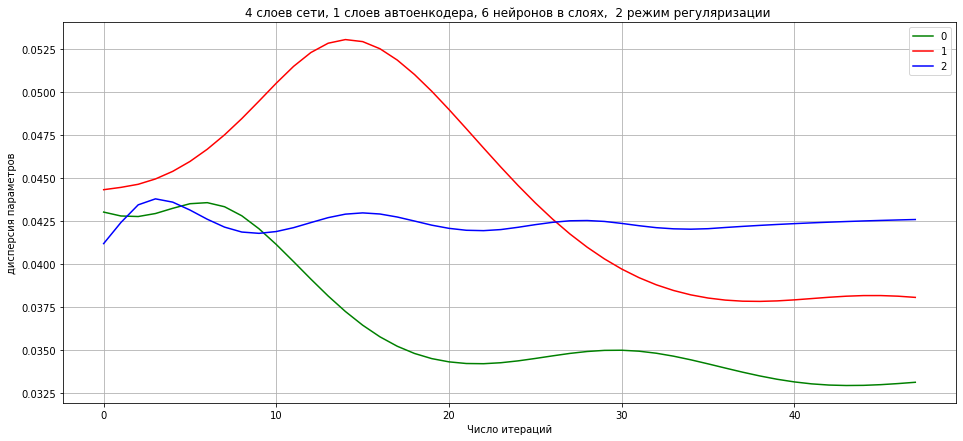
\includegraphics[width=\linewidth]{Green_low.png}}
\caption{При низкой сложности регуляризация может привести к повышению дисперсии }
\end{figure}
\begin{figure}[h!]
\center{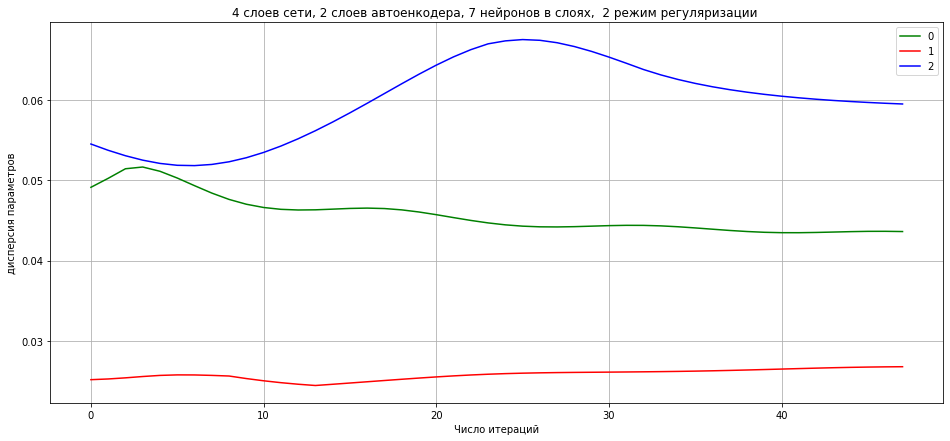
\includegraphics[width=\linewidth]{green_in_middle.png}}
\caption{Одно из расписаний может оказаться неэффективным }
\end{figure}

\newpage

\begin{figure}[h!]
\center{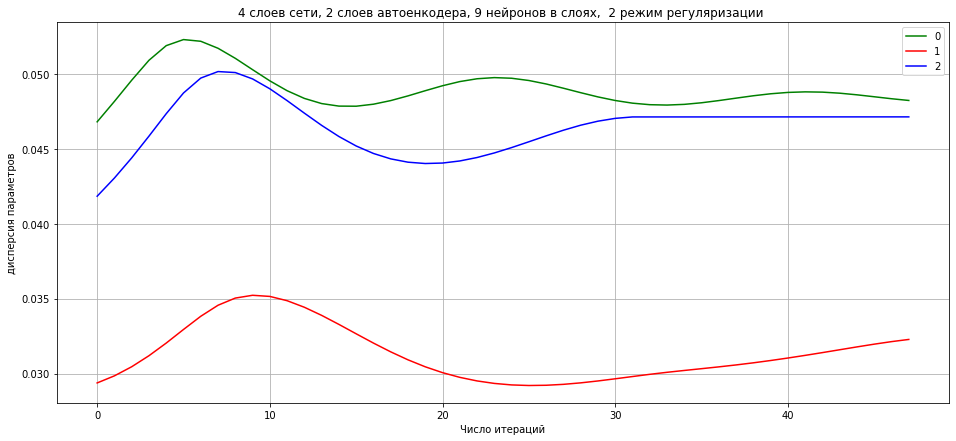
\includegraphics[width=\linewidth]{green_above.png}}
\caption{Обычное поведение -- регуляризованные модели показывают меньшую дисперсию }
\end{figure}
\begin{figure}[h!]
\center{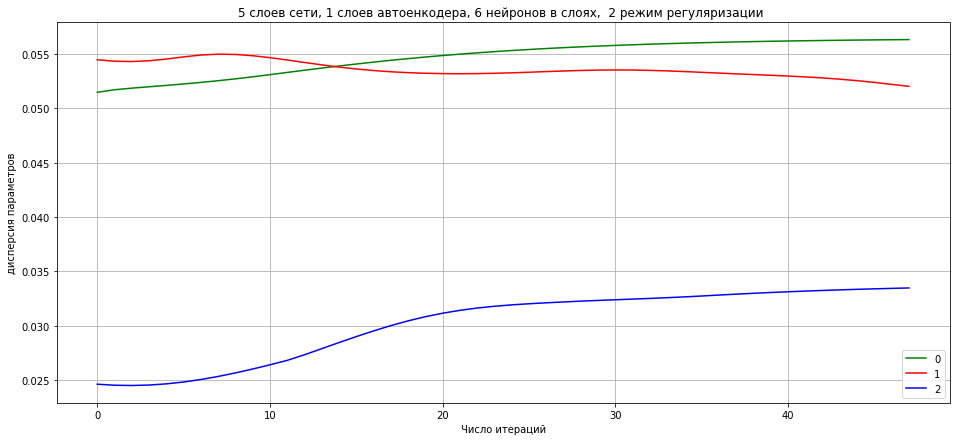
\includegraphics[width=\linewidth]{blue_under.png}}
\caption{Одно из расписаний оказывается эффективнее другого}
\end{figure}

\newpage

\begin{figure}[h!]
\center{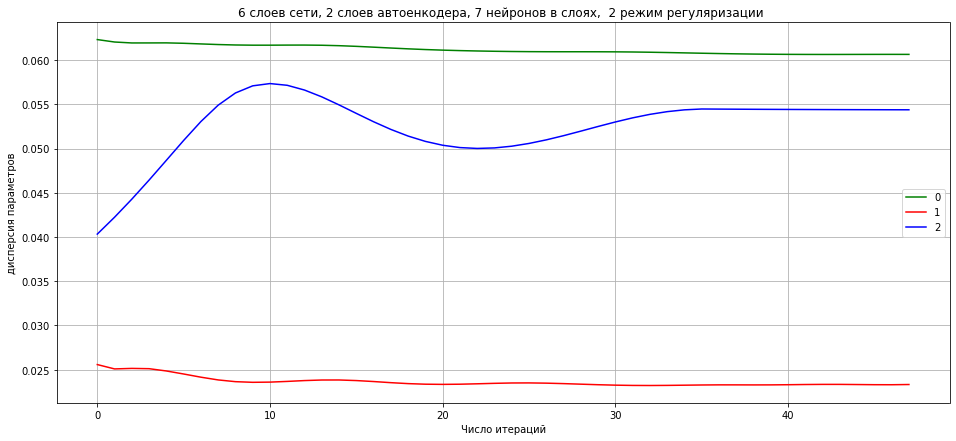
\includegraphics[width=\linewidth]{red_low.png}}
\caption{Одно из расписаний оказывается эффективнее другого}
\end{figure}
\begin{figure}[h!]
\center{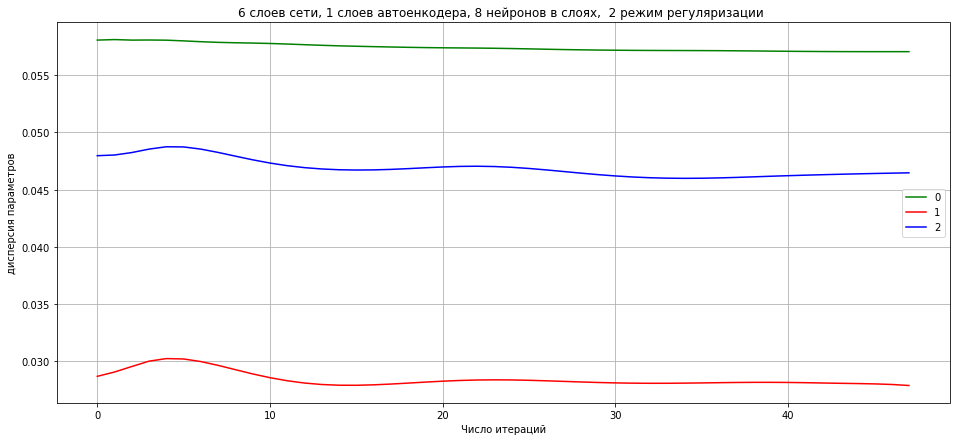
\includegraphics[width=\linewidth]{stable.png}}
\caption{Дисперсия параметров может оказываться постоянной }
\end{figure}

\newpage

      \begin{figure}[h!]
\center{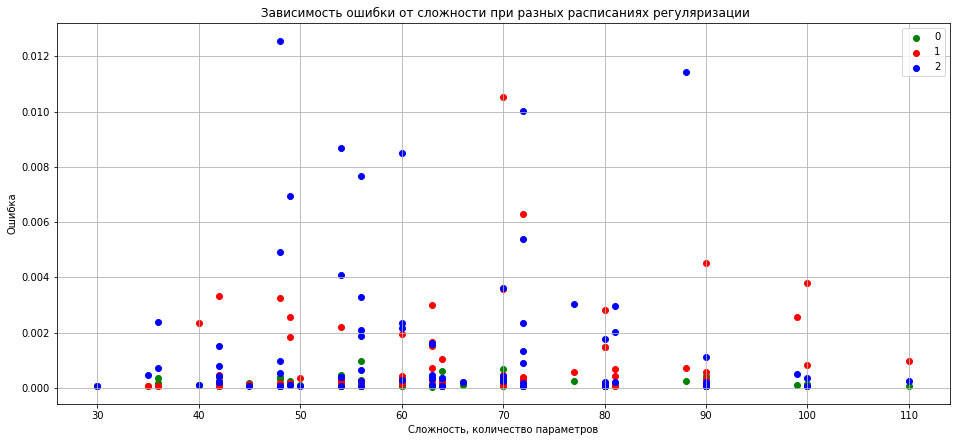
\includegraphics[width=\linewidth]{full_complexity.png}}
\caption{Зависимость ошибки от сложности}
\end{figure}


    
Также была исследована зависимость между сложностью и устойчивостью модели:
      \begin{figure}[h!]
\center{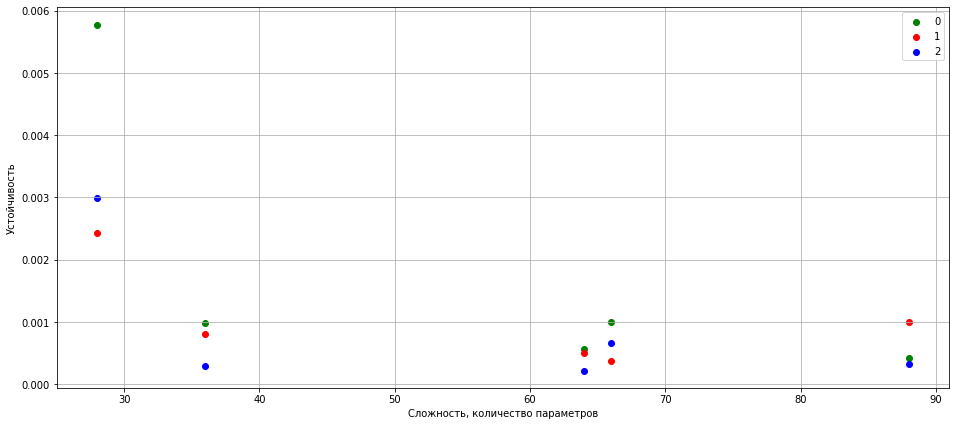
\includegraphics[width=\linewidth]{stability.png}}
\caption{Зависимость между сложностью и устойчивостью}
\end{figure}



Результат : Видим, что с добавленной регуляризацией при равной сложности точность выше. Устойчивость, то есть дисперсия ошибки, меньше при добавленной регуляризации, как и ожидалось.
\section{Заключение}


\section{Supplementary}

Линейная или логистическая регрессия и один нейрон~--- имеют вид
\begin{equation}\label{eq11}
f(\xb,\wm)=\sigmab(\wm^\mathsf{T}\xb),
\end{equation}
где $\sigmab$~---~ функция активации, непрерывная монотонная дифференцируемая функция~(\ref{eq49}),  $\wm$~---~ вектор параметров, $\xb$~---~объект, вектор с присоединенным элементом единица соответствующим аддитивному параметру $w_0$. При использовании линейной функции активации,  получаем линейную регрессию $f(\xb,\wm)=\wm^\mathsf{T}\xb.$

Такую функцию активации мы обозначим $\sigmab = \textbf{id} $. При использовании сигмоидной функции активации,  получаем модель логистической регрессии \begin{equation}\label{eq49}
f(\xb,\wm)=\sigma(\wm^\mathsf{T}\xb)=\frac{1}{1+\exp(-\wm^\mathsf{T}\xb)} .
\end{equation}

Двухслойная нейронная сеть, состоящая из линейной комбинации нейронов, однослойных нейронных сетей
\begin{equation}\label{eq12}
f(\xb,\wm)=\sigma^{(2)}\bigg(\sum_{i=1}^{n_2}w_i^{(2)}\cdot\sigma^{(1)}\Bigg(\sum_{i=1}^{n}w_{ij}^{(1)}x_j+w_{i0}^{(1)}\Bigg)+w_0^{(2)}\bigg) = \sigma\circ \wm^{\mathsf{T}}\sigmab\circ \w\xb.
\end{equation}

Метод главных компонент. Модель допускает вращения признакового пространства, то есть координаты (признаки) преобразовываются только с помощью поворотов:
\begin{equation}
\mathbf{h} = \w\x,
\end{equation}
где $\w$~---~ матрица поворота. Она ортогональна: 
\begin{equation}\label{eq51}
\w\w^\mathsf{T} = \mathbf{I}_n.
\end{equation}
Полученное пространство образов $\mathbf{h}$ называется скрытым. Происходит преобразование без потерь.

При удалении нескольких строк матрицы $\w$, например их число $u < n$,  полученный вектор $\mathbf{h}$ имеет размер $u \times 1$. Получается проекция $\mathbf{h}$ вектора $\mathbf{x}$. Согласно теореме Рао~С.Р.~\cite{fourth}, первые $u$ главных компонент восстанавливают $\mathbf{h}$ оптимальным способом,
\begin{equation}\label{eq45}
\textbf{r}(\textbf{x}) = \w^{\mathsf{T}}\mathbf{h}.
\end{equation}

Автокодировщик $\mathbf{h}$~---~ это монотонное нелинейное отображение входного вектора свободных переменных $\textbf{x} \in \mathbb{R}^n$ в скрытое представление $\mathbf{h} \in \mathbb{R}^{u}$ вида:
\begin{equation}\label{eq52}
\mathbf{h}(\x) = \sigmab(\underset{u \times n}{\w}\x + \mathbf{b}) .
\end{equation}
В случае $\sigmab = \textbf{id}$ и \eqref{eq51} автокодировщик тождественен методу главных компонент. Скрытое представление $\textbf{h}$ реконструирует вектор $\textbf{x}$ линейно:
\begin{equation}\label{eq53}
\mathbf{r}(\x) = \underset{n \times u}{\w{'}}\mathbf{h} + \wm_{0}^{'} .
\end{equation}



\begin{enumerate}[label*=\arabic*.]
    \item
    Lasso или $L_1$ регуляризация вида:
    \[\rk_1(w) = \|w\|_1\]
    \item
    Штраф за количество слоев в нейронной сети:
    \[\rk_2(k) = k\]
    \item
    Штраф за неортогональность матрицы:
    \[\rk_3(W) = \|WW^T - I\|\]
    \item 
    Несколько видов Тихоновской регуляризации:
    \begin{enumerate}[label*=\arabic*.]
        \item
        Ridge или $L_2$ регуляризация вида:
        \[\rk_4(w) = \|w\|_2^2\]
        \item
        Штраф за частоту появления весов
        \[
        A = \frac{1}{3} \begin{bmatrix}
            \frac{2}{3}& \frac{2}{3} & 0 & 0 &0 &0& 0\\
            1 & 1 & 1 & 1& 0 & 0 & 0 \\
            0& 0& 1 & 1& 1 & 0 & 0 \\
            0& 0& 0 & 1& 1 & 1 & 0 \\
            0& 0& 0 & 0& 1 & 1 & 1\\
            0& 0& 0 & 0 & 0& \frac{2}{3}& \frac{2}{3}
        \end{bmatrix}
        \]
        \\
        
        \[\rk_5(W) =  \|(I -A)W\|\]
        \item 
        Штраф за локальную разницу в весах
        \[
        B = \begin{bmatrix}
            -2& 2 & 0 & 0 & 0 &0 &0\\
            -1 & 0 & 1 & 0& 0 & 0 & 0 \\
            0& -1& 0 & 1& 0 & 0 & 0 \\
            0& 0& -1 & 0& 1 & 0 & 0 \\
            0& 0& 0 & -1& 0 & 1 & 0\\
            0& 0& 0 & 0 & 0& -2& 2
        \end{bmatrix}
        \]
        \\
        \[\rk_6(W) =  \|BW\|\]
    \end{enumerate}
\end{enumerate}


Помимо аддитивной регуляризации были разработаны и другие методы. В статье \cite{chernousova2014linear} предлагается алгоритм вычисления ошибки при использовании контроля по отдельным объектам.\\
Задана центрированная нормированная выборка :
\begin{equation}\label{f1}
\left\{\left(\mathbf{x}_{i}, y_{i}\right), i=1, \ldots, N\right\}, \mathbf{x}_{i}=\left(x_{1 i} \cdots x_{n i}\right)^{T} \in \mathbb{R}^{n}, y_{i} \in \mathbb{R}
\end{equation}
\begin{equation}
\sum_{i=1}^{N} \mathbf{x}_{j}=\mathbf{0}, \sum_{i=1}^{N} y_{j}=0, \frac{1}{N} \sum_{i=1}^{N} x_{i j}^{2}=1, i \in I=\{1, \ldots, n\},
\end{equation}
 Задача -- минимизировать вектор \textbf{a}, параметры регрессии $\hat{y}(\mathbf{x})=\wm^{T} \mathbf{x}$:
\begin{equation}
\begin{aligned} J_{\mathrm{NEN}}\left(\wm | \lambda_{1}, \lambda_{2}\right) &=\lambda_{2} \sum_{i=1}^{n} a_{i}^{2}+\lambda_{1} \sum_{i=1}^{n}\left|a_{i}\right|+\sum_{i=1}^{N}\left(y_{j}-\sum_{i=1}^{n} a_{i} x_{i j}\right)^{2} \\ &=\lambda_{2} \wm^{T} \wm+\lambda_{1}\|\wm\|_{1}+(\mathbf{y}-\mathbf{X} \wm)^{T}(\mathbf{y}-\mathbf{X} \wm) \rightarrow \min (\wm) \\ \mathbf{y}=&\left(y_{1} \cdots y_{N}\right) \in \mathbb{R}^{N}, \mathbf{X}=\left(\mathbf{x}_{1} \cdots \mathbf{x}_{N}\right)^{T}(N \times n) \\ \hat{\wm}_{\lambda_{1}, \lambda_{2}} &=\left(\hat{a}_{i, \lambda_{1}, \lambda_{2}}, i \in I\right)=\arg \min J_{\mathrm{NEN}}\left(\wm | \lambda_{1}, \lambda_{2}\right) \in \mathbb{R}^{n} \end{aligned}
\end{equation}

Предлагается следующий подход:
\begin{equation}
\begin{array}{l}{J_{\mathrm{EN}}\left(\wm | \lambda_{1}, \lambda_{2}\right)=\lambda_{2} \sum_{i=1}^{n}\left(a_{i}-a_{i}^{*}\right)^{2}+\lambda_{1} \sum_{i=1}^{n}\left|a_{i}\right|+\sum_{i=1}^{N}\left(y_{j}-\sum_{i=1}^{n} a_{i} x_{i j}\right)^{2}} \\ {\quad=\lambda_{2}\left(\wm-\frac{1}{N} \mathbf{X}^{T} \mathbf{y}\right)^{T}\left(\wm-\frac{1}{N} \mathbf{X}^{T} \mathbf{y}\right)+\lambda_{1}\|\wm\|_{1}+(\mathbf{y}-\mathbf{X} \wm)^{T}(\mathbf{y}-\mathbf{X} \wm) \rightarrow \min (\wm)}\end{array}
\end{equation}
\begin{equation}
\hat{\wm}_{\lambda_{1}, \lambda_{2}}=\left(\hat{a}_{i, \lambda_{1}, \lambda_{2}}, i \in I\right)=\arg \min J_{\mathrm{EN}}\left(\wm | \lambda_{1}, \lambda_{2}\right) \in \mathbb{R}^{n},
\end{equation}
где $\wm^{*}=(1 / N) \mathbf{X}^{T} \mathbf{y}$. Таким образом, можно переписать задачу в следующем виде:
\begin{equation}
\frac{\lambda_{1}}{1+\lambda_{2} / N}\|\wm\|_{1}+\left[\wm^{T} \frac{\mathbf{X}^{T} \mathbf{X}+\lambda_{2} \mathbf{I}}{1+\lambda_{2} / N} \wm-2 \mathbf{y}^{T} \mathbf{X} \wm\right] \rightarrow \min (\wm),
\end{equation}
Вводится разбиение множества параметров по знаку:
\begin{equation}
\left\{\begin{array}{l}
{\hat{I}_{11}^{-}, \lambda_{2}=\left\{i \in I: \hat{a}_{i, \lambda_{1}, \lambda_{2}}<0\right\}} \\
{\hat{I}_{1_{1}, \lambda_{2}}^{0}=\left\{i \in I: \hat{a}_{i, \lambda_{1}, \lambda_{2}}=0\right\}, I=\hat{I}_{\lambda_{1}, \lambda_{2}}^{-} \cup \hat{I}_{\lambda_{1}, \lambda_{2}}^{0} \cup \hat{I}_{\lambda_{1} \lambda_{2}}^{+}} \\
{\hat{I}_{\lambda_{1}^{+}, \lambda_{2}}^{+}=\left\{i \in I: \hat{a}_{i, \lambda_{1}, \lambda_{2}}>0\right\}}
\end{array}\right.
\end{equation}.
После некоторых преобразований:
\begin{equation}
\begin{array}{c}
{\hat{S}_{\mathrm{LOO}}\left(\lambda_{1}, \lambda_{2}\right)=\frac{1}{N} \sum_{k=1}^{N}\left(\hat{\delta}_{k, \lambda_{1}, \lambda_{2}}^{(k)}\right)^{2}} \\
{\hat{\delta}_{k, \lambda_{1}, \lambda_{2}}^{(k)}=y_{k}-\hat{y}_{k, \lambda_{1}, \lambda_{2}}^{(k)}=y_{k}-\tilde{\mathbf{x}}_{k}^{T} \hat{\wm}_{\lambda_{1}, \lambda_{2}}^{(k)}}
\end{array}
\end{equation}
и
\begin{equation}
\hat{S}_{\mathrm{LOO}}^{\mathrm{EN}}\left(\lambda_{1}, \lambda_{2}\right)=\frac{1}{N} \sum_{k=1}^{N}\left(\frac{\hat{\delta}_{k, \lambda_{1}, \lambda_{2}}+\frac{1}{N-1} \lambda_{2}\left(y_{k} q_{k, \lambda_{1}, \lambda_{2}}-h_{k, \lambda_{1}, \lambda_{2}}\right)}{1-q_{k, \lambda_{1}, \lambda_{2}}}\right)^{2}(\text {ElasticNet})
\end{equation}
\begin{equation}
\begin{aligned}
&q_{k, \lambda_{1}, \lambda_{2}}=\tilde{\mathbf{x}}_{k}^{T}\left(\tilde{\mathbf{X}}_{\lambda_{1}, \lambda_{2}}^{T} \tilde{\mathbf{X}}_{\lambda_{1}, \lambda_{2}}+\lambda_{2} \tilde{\mathbf{I}}_{\hat{n}_{\lambda_{1}, \lambda_{2}}}\right)^{-1} \tilde{\mathbf{x}}_{k}\\
&h_{k, \lambda_{1}, \lambda_{2}}=\tilde{\mathbf{x}}_{k}^{T}\left(\tilde{\mathbf{X}}_{\lambda_{1}, \lambda_{2}}^{T} \tilde{\mathbf{X}}_{\lambda_{1}, \lambda_{2}}+\lambda_{2} \tilde{\mathbf{I}}_{\hat{n}_{\lambda_{1}, \lambda_{2}}}\right)^{-1} \tilde{\wm}^{*}
\end{aligned}
\end{equation}




\bibliographystyle{unsrt}
\bibliography{References}


\end{document}

